\section{Method}

% --- COPIED FROM ABSTRACT ASSIGNMENT --- %
% Explain your study design, illustrate how the study's results will provide
% evidence for/against your hypothesis, and how the question, hypothesis, and
% study all line up. We encourage you to mirror/copy/adapt other researchers
% methods (e.g. by drawing from the class readings) whenever appropriate (and
% not when it isn't appropriate).

% There are three major points you should hit here.

% Study design:
% What are you going to do? Be detailed and precise.

% Ecological Validity:
% Why does your study answer your research question? Why
% does your evaluation address your hypothesis? Make sure your study, and the
% variables you're measuring, properly address the question you are asking.

We gathered 10 participants from around our department's building and from the
local Hillcrest community.
%
We required that participants be able to read some Haskell code.

\subsection{Measures}

For each participant, we measured:
\begin{itemize}
    \item Time-to-correct solution (per task)
    \item Count of incorrect selections (per task)
    \item Count and type of interpreter queries (across all tasks)
\end{itemize}

The first metric directly tests the hypothesis that examples improve
selection speed, but the result could be misleading if there was also a
change in selection accuracy.
%
Counting incorrect guesses ensures that any such change is captured.
%
Beyond assessing the effectiveness of examples, measuring how often and why
participants used the interactive interpreter provides insight into any
behavior changes that might occur.

\subsection{Trials}
We had two variants.
%
The control version of the tool only showed programs that matched a type signature.
%
The treatment version showed three input-output examples with each program
suggested by the synthesizer.

Each participant went through one training task and four trial tasks.
%
The task was to find the best implementation of a type signature and a
description of what the program should do.
%
Timing began as soon as they were handed a card containing the task, and ended
when they pointed out the correct solution.
%
There was one correct answer per task---and task 3 had no correct solution.
%
Each participant was in a single variant for the entirety of their tasks.

\begin{figure*}[t!]
    \centering
    \begin{subfigure}[t]{0.5\textwidth}
        \centering
        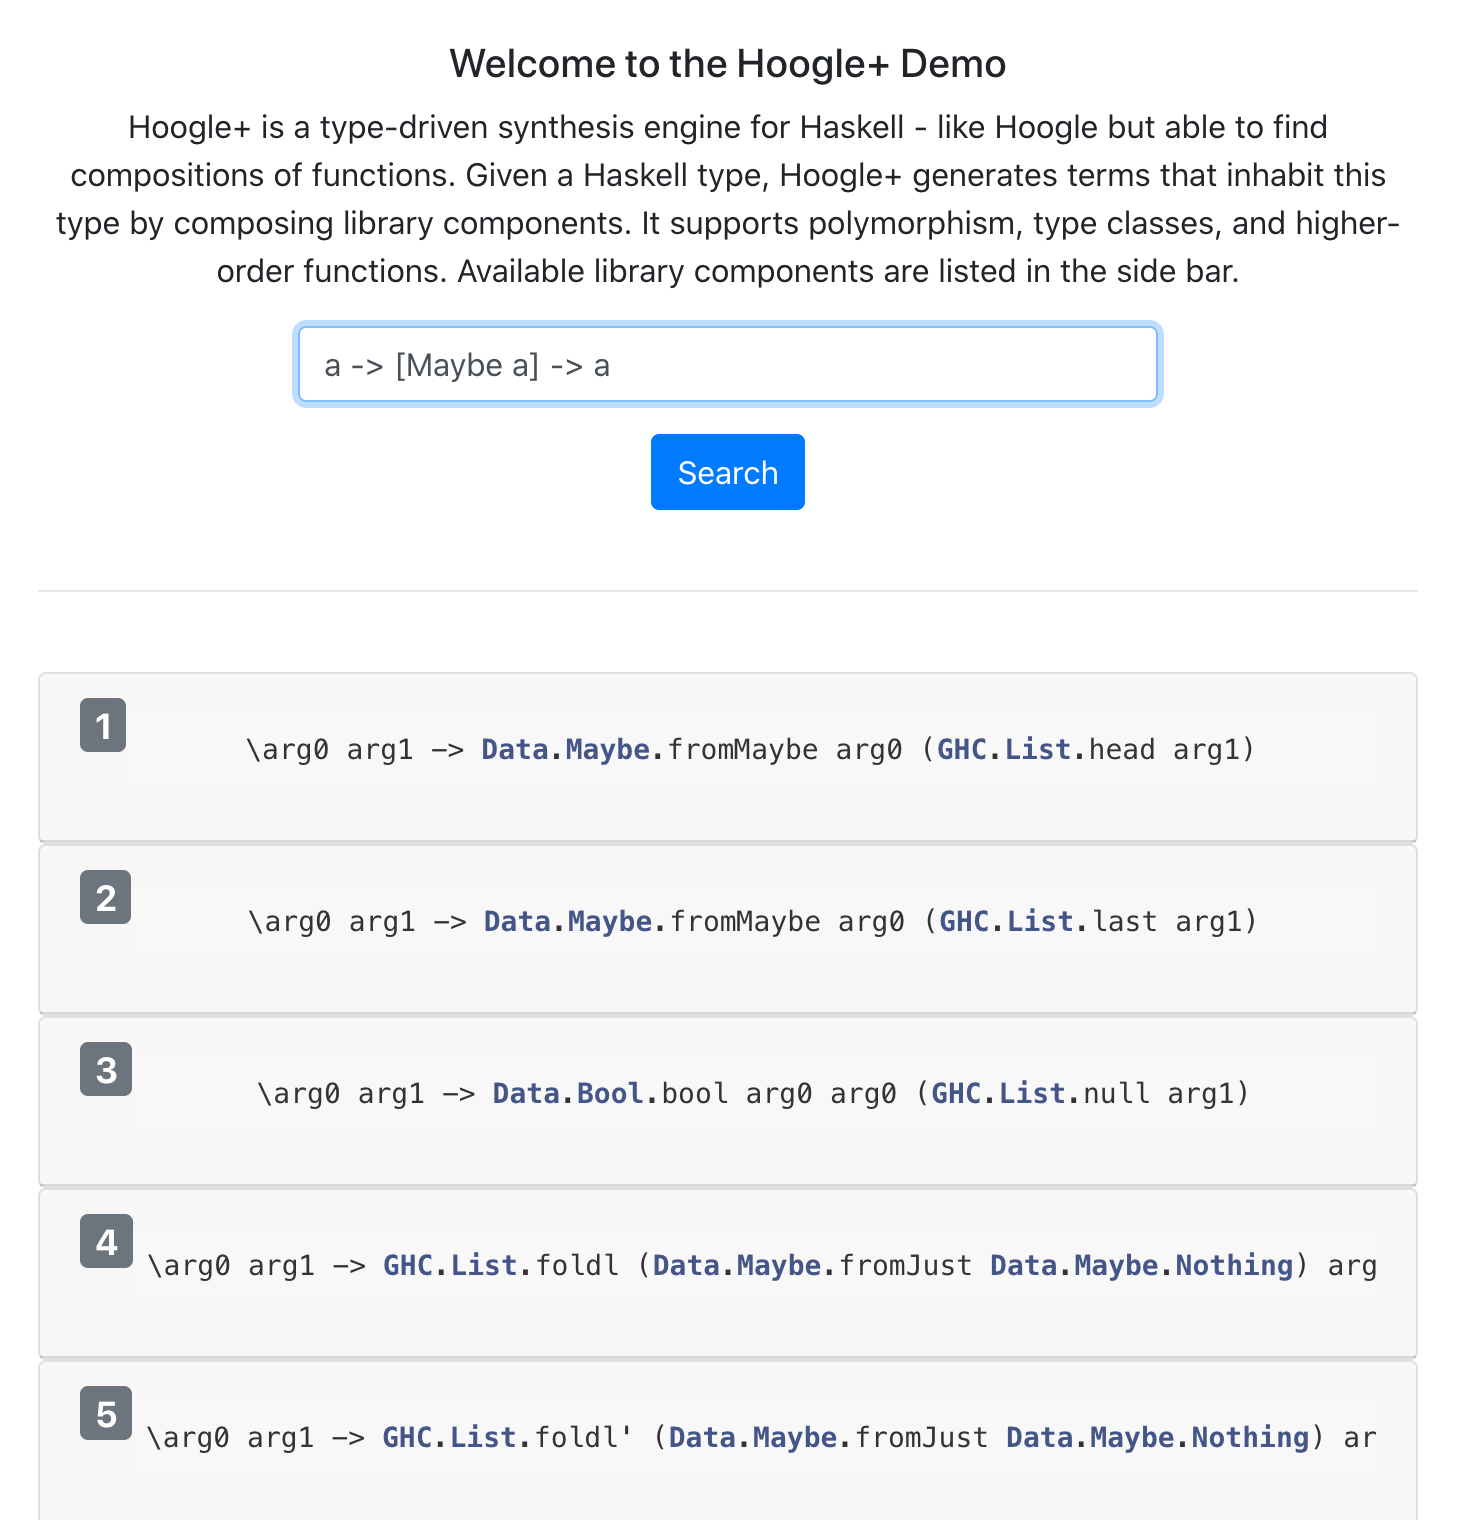
\includegraphics[width=\textwidth]{method/control-ui.png}
        \caption{Control treatment, no examples}
    \end{subfigure}%
    ~
    \begin{subfigure}[t]{0.5\textwidth}
        \centering
        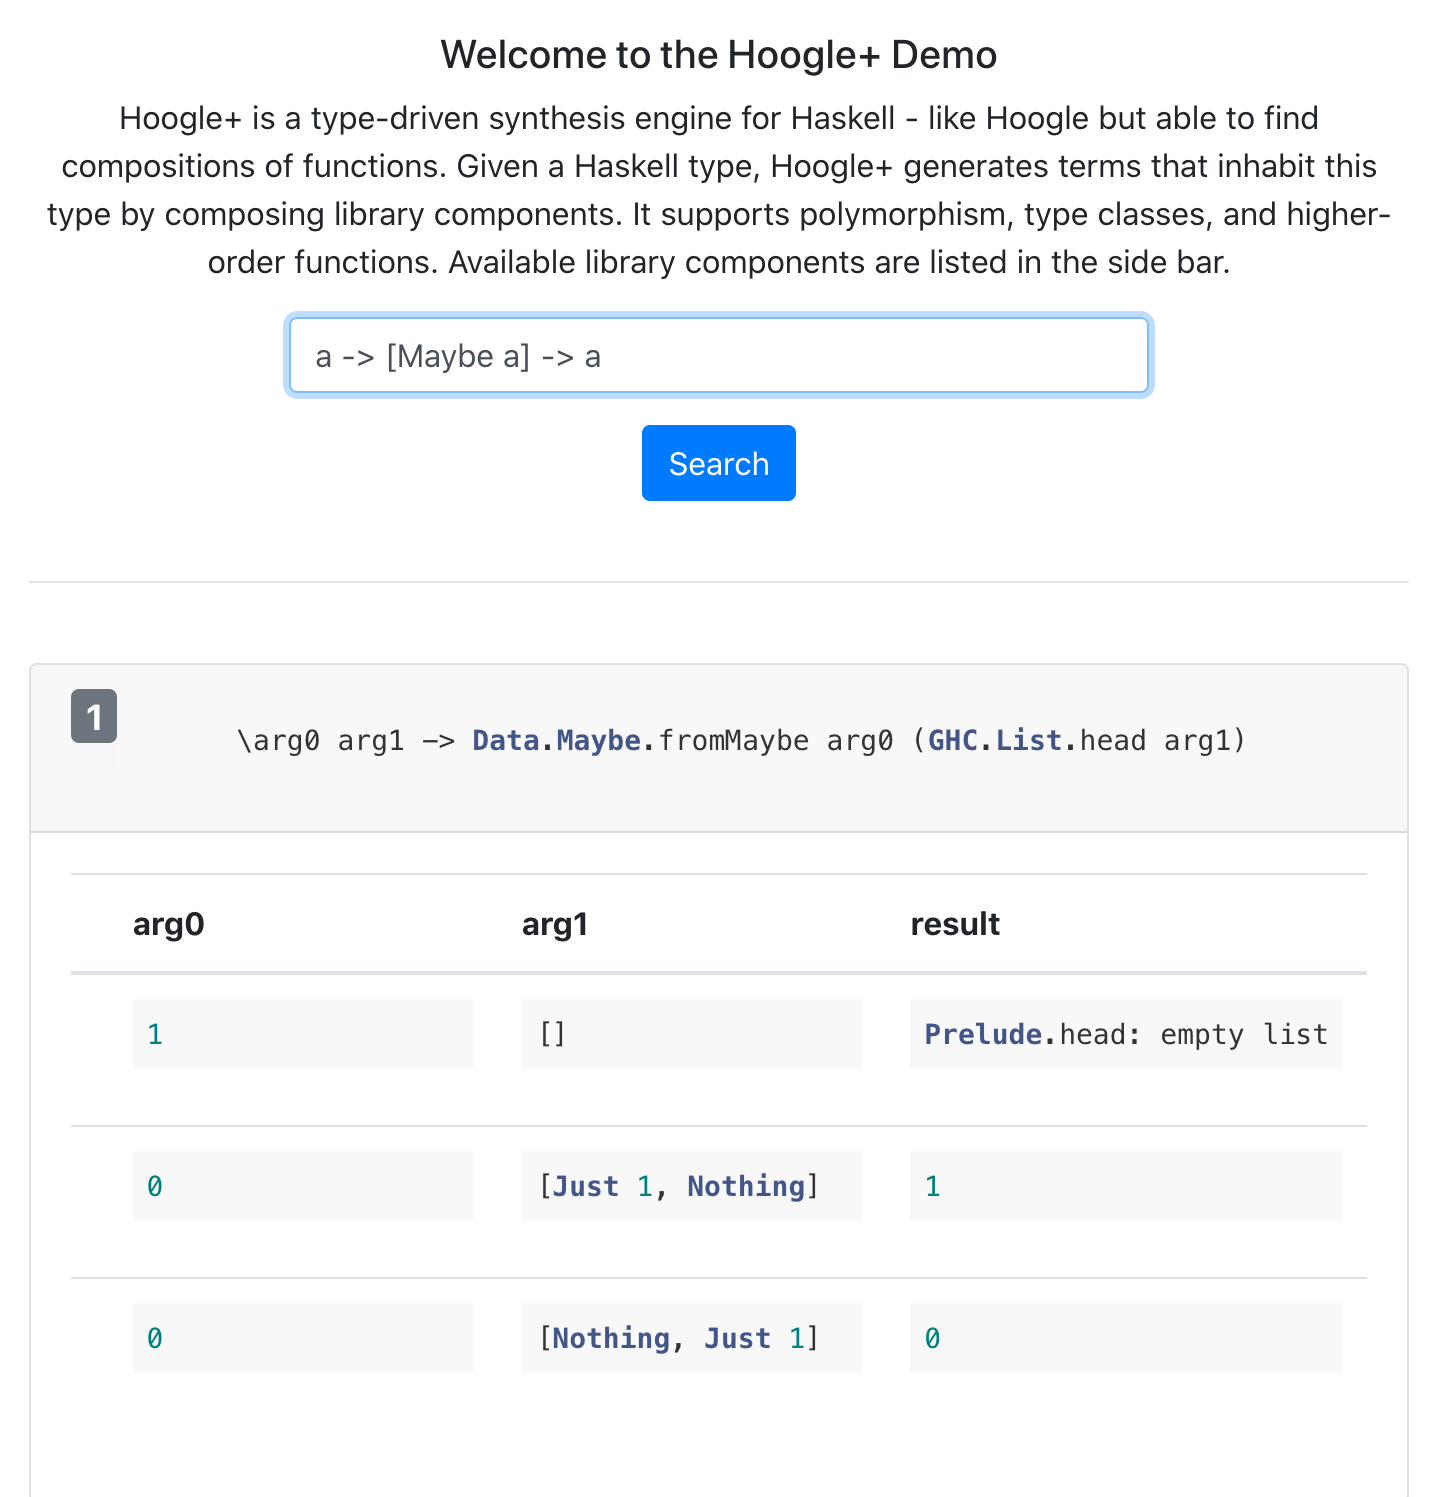
\includegraphics[width=\textwidth]{method/treatment-ui.png}
        \caption{Experimental treatment, examples}
    \end{subfigure}
    \caption{Each participant received one of the two treatments for the duration of the study.}
\end{figure*}